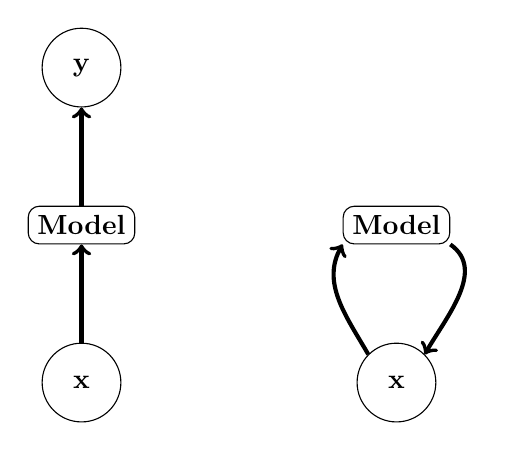
\begin{tikzpicture}


    % \foreach \x in {1,2,3,4}{
    %     \node[circle,draw,fill=white!50, minimum height=10mm,] (Input-\x) at (\intcalcMul{2}{\x},0) {$x_{\x}$};

    %     \node[rectangle, draw, rounded corners, above=of Input-\x] (Model-\x)  {Model};

    %     \node[circle,draw,fill=white!50, minimum height=10mm, above=of Model-\x] (Input-\x) {$y_{\x}$};

    % }

    \node[circle,draw,fill=white!50, minimum height=10mm,] (Input) at (0,0) {$\mathbf{x}$};

    \node[rectangle, draw, rounded corners] (Model) at (0,2)  {\textbf{Model}};

    \node[circle,draw,fill=white!50, minimum height=10mm] at (0,4) (Output) {$\mathbf{y}$};

    \draw[->, line width=1.5] (Input.north) -- (Model.south);

    \draw[->, line width=1.5] (Model.north) -- (Output.south);


    \node[circle,draw,fill=white!50, minimum height=10mm,] (Input-U) at (4,0) {$\mathbf{x}$};

    \node[rectangle, draw, rounded corners] (Model-U) at (4,2)  {\textbf{Model}};

    \draw[->, line width=1.5] (Input-U.north west)  to[out=120, in=-120] (Model-U.south west);

    \draw[->, line width=1.5] (Model-U.south east)  to[out=-35, in=60] (Input-U.north east);
    % \node[right=of Input-15, align=right] {
    % \textbf{Original Input}
    % };
    % \node[right=of Stack-4, align=right] {
    % \textbf{Stacked Input}
    % };

\end{tikzpicture}%